% Overleaf: 默认 pdfLaTeX 编译器直接 Recompile，无需改任何设置。
\documentclass[11pt,a4paper]{article}

% ── Chinese support (CJKutf8, bundled with TeX Live since 2008) ──
\usepackage[T1]{fontenc}
\usepackage[utf8]{inputenc}
\usepackage{CJKutf8}

% ── Layout ──
\usepackage[margin=2.2cm]{geometry}
\usepackage{setspace}
\onehalfspacing

% ── Graphics ──
\usepackage{graphicx}
\usepackage{xcolor}
\usepackage{tikz}
\usetikzlibrary{arrows.meta, positioning, shapes.geometric, calc, backgrounds}

% ── Tables ──
\usepackage{booktabs}
\usepackage{tabularx}
\usepackage{array}

% ── Code ──
\usepackage{listings}
\lstset{
  basicstyle=\small\ttfamily,
  breaklines=true,
  frame=single,
  framesep=4pt,
  rulecolor=\color{gray!40},
  backgroundcolor=\color{gray!5},
  showstringspaces=false,
  aboveskip=6pt,
  belowskip=6pt,
  extendedchars=true,
}

% ── Headers ──
\usepackage{fancyhdr}
\pagestyle{fancy}
\fancyhf{}
\fancyhead[L]{\small\scshape LLM Hypothesis Citation Agent}
\fancyhead[R]{\small\scshape Technical Report}
\fancyfoot[C]{\thepage}
\renewcommand{\headrulewidth}{0.4pt}

% ── Misc ──
\usepackage{caption}
\usepackage{enumitem}
\usepackage{hyperref}
\hypersetup{colorlinks=true, linkcolor=blue!50!black, urlcolor=blue!60!black}

\title{\bfseries\large LLM Hypothesis Citation Agent\\[4pt]\normalsize\mdseries 引文幻觉审计系统 · 技术架构报告}
\author{
    \begin{tabular}[t]{cc}
        刘炎男 & 郭耀远 \\
        \texttt{12311122@mail.sustech.edu.cn} & \texttt{12312902@mail.sustech.edu.cn} \\[1em]
        \multicolumn{2}{c}{齐佳男} \\
        \multicolumn{2}{c}{\texttt{12311812@mail.sustech.edu.cn}}
    \end{tabular}
}
\date{\today}

\begin{document}
\begin{CJK*}{UTF8}{gbsn}

\maketitle
\thispagestyle{empty}
\vspace{-18pt}

% ════════════════════════════════════
\section{引文幻觉验证系统概览}
% ════════════════════════════════════

大语言模型在生成科学假设时会附带引用文献来支撑其主张，但这些引文存在幻觉风险——模型可能编造不存在的论文、虚构 DOI、或将真实文献的内容张冠李戴。本系统是一个针对此类引文幻觉的后审计管道：它不关心假设本身是如何生成的，只关心假设所依赖的引文是否真实存在、元数据是否正确、以及被引文献的内容是否确实支撑模型所声称的主张。

系统的输入来自 DeepScientist\footnote{https://github.com/ResearAI/DeepScientist}——一个开源的科学发现代理框架，以 Claude 作为推理后端，读取论文 PDF、检索相关文献、生成研究假设并以 JSON 格式输出引文主张。DeepScientist 在此仅作为上游数据源，其内部实现不在本系统的关注范围内。本系统的核心价值在于下游：对每一���引文主张进行独立于 LLM 的事实核验。

整体管道为五阶段流水线：

\begin{enumerate}[leftmargin=*,nosep]
  \item \textbf{输入接收}：从 DeepScientist 输出的 claims JSON 中提取每条引文主张及其被引文献元数据（标题、作者、年份、DOI、检索来源）。
  \item \textbf{规范化与富化}：Claims Normalizer 将多格式输出统一为验证器所需的规范 schema；Claims Enricher 利用源论文元数据补全匹配引文的缺失字段。
  \item \textbf{逐条引文审计}：CitationVerifier 对每条 claim 执行四个 API 的交叉验证——存在性查找、元数据比对、支撑度评分——最终赋予 Green（材料明确支撑）、Yellow（合理推断但未直接证明）或 Red（证据不足）标签。
  \item \textbf{多模型平行评审}：四位不同提供商的 LLM 作为平行评审者，独立对完整审计结果评分（1--6 分），评分受确定性上限约束。
  \item \textbf{跨运行记忆归档}：每次审计的引文标签历史、API 可靠性统计和评审决策写入持久化 JSONL 记忆，用于跨运行幻觉模式识别。
\end{enumerate}

在批处理层面，系统在 15 篇跨领域真实论文上进行了泛化压力测试，覆盖 NLP、医学影像、量化金融、物理学、材料科学、神经科学、机器人、气候遥感、教育等学科，验证了审计管道在不同领域引文模式下的稳定性。

\begin{figure}[htbp]
\centering
\begin{tikzpicture}[
  node distance=0.55cm,
  box/.style={rectangle, draw, rounded corners=3pt, fill=blue!3,
              text width=5.0cm, align=center, minimum height=0.72cm, font=\small},
  arrow/.style={-{Stealth[scale=0.9]}, thick},
]
  \node[box, fill=orange!8] (paper) {arXiv PDF 输入（15 篇跨领域论文）};
  \node[box, fill=orange!5, below=of paper] (ds) {DeepScientist 生成假设与引文主张（上游数据源）};
  \node[box, fill=green!8, below=of ds] (audit) {CitationVerifier · 逐条引文审计（存在性 + 元数据 + 支撑度）};
  \node[box, fill=blue!8, below=of audit] (mr) {Multi-Reviewer · 4 模型平行评分（1--6 分，Cap 约束）};
  \node[box, fill=orange!5, below=of mr] (mem) {Research Memory · 跨运行幻觉模式归档};

  \draw[arrow] (paper) -- (ds);
  \draw[arrow] (ds) -- (audit);
  \draw[arrow] (audit) -- (mr);
  \draw[arrow] (mr) -- (mem);
\end{tikzpicture}
\caption{引文幻觉审计管道：从论文输入到跨运行记忆归档的五阶段流程。系统的核心在第三、第四阶段——确定性验证与多模型评审——而非假设生成本身。}
\label{fig:path2}
\end{figure}

% ════════════════════════════════════
\section{引文验证管道}
% ════════════════════════════════════

\subsection{上游：假设与引文的来源}

系统接收的 claims 数据可以来自两条路径。主路径使用 DeepScientist 作为代理，由 Claude 运行器读取论文、检索文献、生成假设并输出结构化 JSON。回退路径使用本地 CitationAuditClaimsGenerator，在 DeepScientist 不可用时通过 PdfReaderTool + LiteratureSearcher + HypothesisGenerator 本地生成。无论来源如何，所有引文主张在进入验证管道前均经过 Claims Normalizer 归一化为统一 schema。

需要强调的是，系统对假设的生成策略不作评判——假设是否新颖、方法论是否合理，这些问题由后续的 Multi-Reviewer 从证据质量角度间接评估。验证管道的唯一任务是逐条核验每条引文主张的事实准确性。

\subsection{核心：确定性引文验证}

CitationVerifier 是系统的核心组件，对每条 claim 执行四阶段检查，全程不依赖 LLM 判断：

\begin{enumerate}[leftmargin=*,nosep]
  \item \textbf{存在性查找}：通过 DOI 或标题在 Crossref、OpenAlex、Semantic Scholar 和 arXiv 四个公共 API 上查询。DOI 精确查找优先，未命中则按标题搜索，结果按引用数降序排列。
  \item \textbf{版本消歧}：当同一文献在多个数据源存在不同记录时（如 preprint 与正式发表版本），按 DOI 精确匹配优先、标题-作者相似度次之的规则合并去重。
  \item \textbf{元数据比对}：综合评估标题文本相似度、作者 Jaccard 重叠度、发表年份差异和 DOI 精确匹配，判断被引文献的元数据是否与公开记录一致。
  \item \textbf{支撑度评分}：将被引文献的 abstract 或 snippet 与 claim 文本进行句子级覆盖分析，计算文本重叠分数和关键词覆盖率，检测是否存在数值矛盾或条件冲突等硬性错误。
\end{enumerate}

综合打分后，每条 claim 归入三级标签：

\begin{itemize}[leftmargin=*,nosep]
  \item \textbf{Green（材料明确支撑）}：文献在公共 API 上确认存在、元数据匹配、abstract 文本直接支撑 claim 主张。需通过九条件 Green Gate 全部判定。
  \item \textbf{Yellow（合理推断但未直接证明）}：文献存在且元数据基本匹配，但 abstract 对 claim 的支撑是间接的、部分的或不确定的。例如 claim 声称某个方法有效，被引文献提出了该方法但未提供实验验证。
  \item \textbf{Red（证据不足）}：文献未找到、DOI 无效、元数据严重不匹配，或存在硬性矛盾（如 claim 声称的数值与文献记录不一致）。
\end{itemize}

\subsection{LLM 的使用边界}

LLM 在整个验证管道中仅在两个环节被调用：上游的 HypothesisGenerator 中用于生成假设（创造性任务），以及 CitationVerifier 中可选的单句解释生成（仅用于人工阅读参考，内部约束不得据此修改标签）。所有真值判断——引文是否存在、元数据是否正确、abstract 是否支撑主张——均由确定性 API 查询和规则判定完成。这一设计选择基于实测观察：LLM 在事实核验任务上存在确认偏误，倾向于将听上去合理的引文标记为真实。

% ════════════════════════════
\section{Tool-Use 双层架构}
% ════════════════════════════

系统的工具调用采用双层设计：上游代理层使用 LLM 函数调用自主检索文献以生成假设，下游验证层使用确定性 API 查询完成逐条引文的事实核验。两层通过工作流编排器衔接，所有工具调用的输入输出和耗时全量记录到审计日志。

\subsection{代理层：LLM 驱动的文献检索}

HypothesisGenerator 是系统中唯一使用 LLM 函数调用的组件。它注册一个 \texttt{search\_literature} 工具——接受搜索查询字符串数组、返回学术论文元数据。代理循环限制为最多三轮：LLM 接收论文摘要后自主决定是否调用工具；若调用，工作流提取查询参数，通过 LiteratureSearcher 依次查询 Crossref、OpenAlex、Semantic Scholar 和 arXiv，合并去重后以 tool message 格式回传结果；LLM 评估后决定继续搜索或输出最终 JSON。三轮结束后强制输出结构化结果。

\subsection{验证层：四个公共 API 的交叉查询}

CitationVerifier 不使用 LLM 函数调用。四个查询函数分别封装 Crossref、OpenAlex、Semantic Scholar 和 arXiv 的 HTTP 请求，按固定管道顺序执行：Lookup → Version Resolution → Metadata Matching → Support Scoring → Classification。LLM 仅用于生成人类可读的审核说明，不参与判定。

\subsection{审计追踪}

每次工具调用都通过 ToolCallLogger 写入 tool\_calls.jsonl（含调用 ID、时间戳、工具名、耗时、状态和错误信息）。EvidenceStore 将各工具产出的证据项以证据 ID 关联回对应的工具调用，写入 evidence\_items.jsonl。两个日志共同构成从工具调用到证据项的完整审计链路。

\begin{figure}[htbp]
\centering
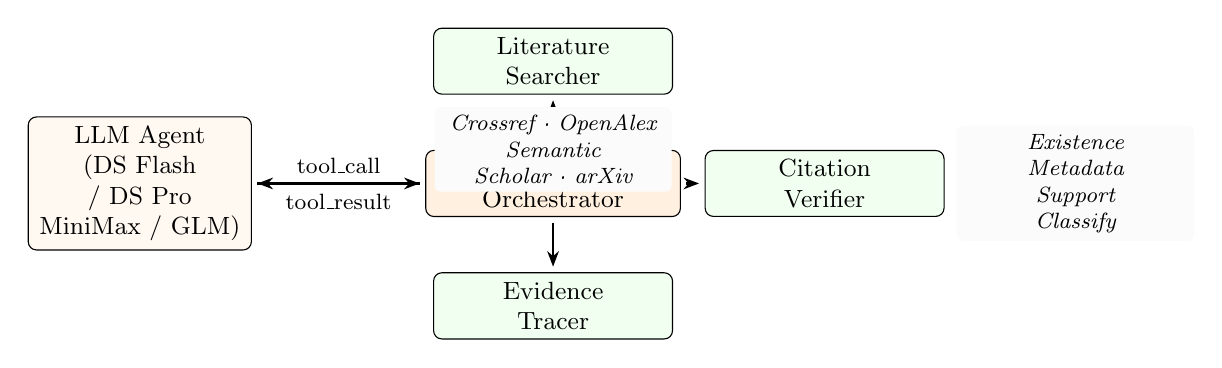
\begin{tikzpicture}[
  node distance=0.5cm and 1.5cm,
  box/.style={rectangle, draw, rounded corners=3pt, fill=blue!4,
              text width=2.8cm, align=center, minimum height=0.75cm, font=\small},
  tool/.style={rectangle, draw, rounded corners=3pt, fill=green!6,
               text width=2.8cm, align=center, minimum height=0.70cm, font=\small},
  apinote/.style={font=\footnotesize\itshape, text width=2.8cm, align=center, fill=gray!3,
                  inner sep=3pt, rounded corners=2pt},
  arrow/.style={-{Stealth[scale=0.85]}, thick, shorten >=2pt, shorten <=2pt},
  dasharrow/.style={-{Stealth[scale=0.85]}, thick, dashed, shorten >=2pt, shorten <=2pt},
]
  \node[box, fill=orange!12, text width=3.0cm, minimum height=0.8cm] (wf) {Workflow\\Orchestrator};
  \node[box, fill=orange!5, text width=2.6cm, left=2.2cm of wf] (llm) {LLM Agent\\(DS Flash / DS Pro\\ MiniMax / GLM)};
  \node[tool, above=0.7cm of wf] (lit) {Literature\\Searcher};
  \node[tool, right=0.3cm of wf] (cv) {Citation\\Verifier};
  \node[tool, below=0.7cm of wf] (et) {Evidence\\Tracer};

  \draw[arrow] (llm) -- node[above, font=\footnotesize]{tool\_call} (wf);
  \draw[dasharrow] (wf) -- node[below, font=\footnotesize]{tool\_result} (llm);
  \draw[arrow] (wf) -- (lit);
  \draw[arrow] (wf) -- (cv);
  \draw[arrow] (wf) -- (et);

  \node[apinote, below=0.15cm of lit] {Crossref · OpenAlex\\Semantic Scholar · arXiv};
  \node[apinote, right=0.15cm of cv] {Existence\\Metadata\\Support\\Classify};
\end{tikzpicture}
\caption{双层工具调用架构。左侧 LLM Agent 使用函数调用检索文献（虚线表示 3 轮循环），右侧验证层以确定性 API 查询逐条核验引文事实。}
\label{fig:tool_arch}
\end{figure}

% ════════════════════════════════
\section{Research Memory 双层记忆}
% ════════════════════════════════

系统包含两套独立的记忆机制，分别面向不同时间尺度的幻觉风险。ResearchMemory 以文件持久化追踪跨运行引文可靠性；AgentMemory 以层级结构记录代理行为模式并自动归并为长期规则。

\subsection{ResearchMemory：跨运行引文审计记忆}

ResearchMemory 是基于 JSONL 的持久化存储，覆盖五类文件：

\begin{itemize}[leftmargin=*,nosep]
  \item \textbf{Citation Memory}：按 DOI 或规范化标题键 upsert，累积每次运行中该引文的标签历史（label\_history）和最新标签（latest\_color\_label）。
  \item \textbf{Provider Memory}：记录各数据源在每次运行中的成功/失败/错误计数。
  \item \textbf{Reviewer Memory}：追加式记录每次多评审面板的评分和决策（append-only，每轮评审均视为独立历史证据）。
  \item \textbf{Failure Memory}：按复合键 upsert，存储 Yellow/Red 级别的引文风险项及 case 级失败记录。
  \item \textbf{Case Memory}：记录每个 case 每次运行的 Green/Yellow/Red 分布和最终评分。
\end{itemize}

跨运行反幻觉的三个机制：其一，当某 DOI 在历史运行中曾被标记为 Red，Multi-Reviewer 会收到完整标签历史作为评审上下文；其二，跨运行累积的 API 错误计数帮助识别不可靠数据源；其三，merge\_label\_history 确保历史标签不被覆盖，latest\_color\_label 反映最新运行结果。

\subsection{AgentMemory：层级化反思记忆}

AgentMemory 采用 Working / Short-term / Long-term 三层架构。Working Memory 记录单次运行的计数器；Short-term Memory 积累近期的成功经验和验证错误；当某类错误累积超过 30 条时自动压缩为 Long-term rule；成功模式出现三次以上则晋升为 Long-term success\_pattern。反思数据中记录了三类高频幻觉：元数据伪造、过度推断、引文无关——这些反思注入系统提示使代理携带对过往错误的记忆。

\begin{figure}[htbp]
\centering
\begin{tikzpicture}[
  node distance=0.45cm,
  box/.style={rectangle, draw, rounded corners=3pt, fill=blue!5,
              text width=5.0cm, align=center, minimum height=0.72cm, font=\small\bfseries},
  listbox/.style={rectangle, draw, rounded corners=3pt, fill=orange!3,
                  text width=5.0cm, align=left, minimum height=0.65cm,
                  font=\footnotesize, inner sep=4pt},
  arrow/.style={-{Stealth[scale=0.85]}, thick},
]
  \node[box, fill=orange!12] (rm) {ResearchMemory · 跨运行 · 持久 · JSONL};
  \node[listbox, below=of rm] (rm1) {citation: upsert by DOI/title, 累积 label\_history};
  \node[listbox, below=of rm1] (rm2) {provider: upsert, API 成功/失败计数};
  \node[listbox, below=of rm2] (rm3) {reviewer: append-only, 每轮评审独立存档};
  \node[listbox, below=of rm3] (rm4) {failure: upsert by compound key};
  \node[listbox, below=of rm4] (rm5) {case: upsert by case\_id|run\_id};

  \draw[arrow] (rm) -- (rm1);

  \node[box, fill=blue!12, right=1.4cm of rm] (am) {AgentMemory · 单会话 · 层级 · 反思};
  \node[listbox, below=of am, fill=blue!3] (am1) {Working: per-run counters (DOI/Green/Yellow/Red 计数)};
  \node[listbox, below=of am1, fill=blue!3] (am2) {Short-term: 近期 success + verification\_error 经验};
  \node[listbox, below=of am2, fill=blue!3] (am3) {auto-compress (30+ errors / 3+ successes)};
  \node[listbox, below=of am3, fill=blue!3] (am4) {Long-term: verification\_rules + provider\_insights};
  \node[listbox, below=of am4, fill=blue!3] (am5) {Long-term: success\_patterns};

  \draw[arrow] (am) -- (am1);

  \node[font=\footnotesize, above=0.05cm of rm, align=center, fill=orange!8, inner sep=2pt] {目标：跨运行引文可靠性};
  \node[font=\footnotesize, above=0.05cm of am, align=center, fill=blue!8, inner sep=2pt] {目标：单代理行为纠偏};
\end{tikzpicture}
\caption{双层记忆架构。左侧 ResearchMemory 追踪跨运行引文级一致性，右侧 AgentMemory 纠正单代理行为偏差。}
\label{fig:memory_arch}
\end{figure}

% ════════════════════════════════════
\section{Multi-Reviewer 多模型平行评审}
% ════════════════════════════════════

Multi-Reviewer 是运行于确定性引文验证之后的评分面板。它对完整假设包中的每条引文审计结果进行综合评分，产出 1--6 分的最终分值和 Accept / Revise / Reject 三级决策。其核心约束是：确定性验证结果（Green/Yellow/Red 标签分布）在评分上具有优先权——LLM 评审不能通过高估计分来掩盖引文层面的证据缺陷。

\subsection{评分体系：证据质量三阶梯}

Multi-Reviewer 的 1--6 评分直接对应引文的证据支撑质量，而非假设的新颖性或方法论合理性：

\begin{table}[htbp]
\centering
\caption{评分与证据质量对照}
\begin{tabularx}{\textwidth}{@{}ccl>{\raggedright\arraybackslash}X@{}}
\toprule
\textbf{分数} & \textbf{标签} & \textbf{证据等级} & \textbf{含义} \\
\midrule
1--2 & Red   & 证据不足   & 引文未在公共 API 上找到，或 DOI 无效，或元数据与被引文献严重不匹配，或存在硬性数值矛盾。假设的主张缺乏可验证的文献支撑。 \\
3--4 & Yellow & 合理推断但未直接证明 & 引文在公共 API 上确认存在，元数据基本匹配，但被引文献的 abstract 或全文对 claim 主张的支撑是间接的、部分的或推测性的。例如 claim 声称某方法在特定条件下有效，但被引文献仅提出了方法而未经实验验证。 \\
5--6 & Green  & 材料明确支持 & 引文确认存在，元数据完全匹配，被引文献的 abstract 或全文直接、明确地支撑 claim 主张。九条件 Green Gate 全部通过。 \\
\bottomrule
\end{tabularx}
\end{table}

分数越高代表引文证据质量越强。评分不是对假设本身优劣的评判，而是对假设所依赖的文献证据链完整性的度量。

\subsection{架构：四模型平行评审}

四位评审被配置为完全平行的通用评审者，使用四种不同模型、三个不同 API 提供商。每位评审基于相同的审计上下文（引文验证 CSV、证据链、API 查询日志、历史记忆命中）独立评分。评审之间不通信、不协调，评分分歧本身即为审计质量的信号。元评审使用 DeepSeek V4 Pro，综合四份独立评分后产出加权最终分数和决策标签。

\begin{table}[htbp]
\centering
\caption{四位平行评审配置}
\begin{tabular}{@{}clllc@{}}
\toprule
\textbf{ID} & \textbf{模型} & \textbf{提供商} & \textbf{API 端点} & \textbf{评审范围} \\
\midrule
R1 & deepseek-v4-flash  & DeepSeek & api.deepseek.com  & 通用评审 \\
R2 & deepseek-v4-pro    & DeepSeek & api.deepseek.com  & 通用评审 \\
R3 & minimax-text-01    & MiniMax  & api.minimax.chat  & 通用评审 \\
R4 & glm-4-flash        & GLM      & open.bigmodel.cn  & 通用评审 \\
\bottomrule
\end{tabular}
\end{table}



\subsection{确定性评分上限（Score Cap）}

为确保 LLM 评审不能通过高估计分掩盖引文层面的证据缺陷，系统基于引文标签分布计算硬性评分上限。Cap 初始值为 6，逐级施加封顶规则，取最低触发上限为有效 Cap：

\begin{table}[htbp]
\centering
\caption{确定性评分上限触发规则}
\begin{tabularx}{\textwidth}{@{}>{\ttfamily}l>{\raggedright\arraybackslash}Xc@{}}
\toprule
\textbf{触发条件} & \textbf{规则说明} & \textbf{上限} \\
\midrule
any\_red\_claim          & 存在任意证据不足（Red）的引文 & 2 \\
red\_line\_error\_type   & 检测到硬性错误（not\_found、DOI 无效、数值矛盾） & 2 \\
yellow\_majority         & 合理推断（Yellow）占比超过 50\% & 4 \\
no\_green\_claims        & 无引文达到材料明确支持（Green）标准 & 4 \\
support\_risk\_error     & 主张过强 / 关键术语缺失 / 数值矛盾 & 4 \\
risk\_penalty\_total     & 确定性风险罚分累计 $\ge 3$ & 4 \\
\bottomrule
\end{tabularx}
\end{table}

Cap 为 2 时，最终分数被限制在 1--2 分（Red 区间），决策强制 Reject——即使 LLM 给出高估分，也不能将证据不足的引文包装为可接受的假设。Cap 为 4 时，最多允许 3--4 分（Yellow 区间），决策限制为 Revise，禁止 Accept。

\subsection{双模式运行与降级策略}

三种运行模式：auto（检测到 API 密钥则用 LLM 评审，否则降级为确定性规则评分）、deepseek（强制 LLM，密钥缺失仍降级）、deterministic（完全跳过 LLM，纯规则评分）。确定性模式基于 Green/Yellow/Red 标签分布直接计算分数区间，确保即使所有外部 API 均不可用，系统仍能产出有依据的评分结果。

\subsection{评审一致性与冲突消解}

四位评审的一致程度由分数极差度量：极差不大于 1 为高一致性，不大于 2 为中一致性，超过 2 为低一致性。极端情况下，即使四位 LLM 全部给出一致的高分，若引文验证中检出 Red 标签，Cap 机制将最终分数截断至 2 分（证据不足），决策强制 Reject。评审共识不能凌驾于确定性事实之上。

% ════════════════════════════
\section{实验统计与可复现结果}
% ════════════════════════════

为避免只展示单次成功案例，本报告对当前项目输出目录中的真实运行产物进行了汇总统计。统计范围包括
15x campaign、20x campaign 和 local runs 三类输出。统计对象不是人工编写的示例数字，
而是已经生成的引文核查表、证据链、工具调用日志和证据记录等可复现文件。

\begin{table}[htbp]
\centering
\caption{三个输出目录的合计审计规模}
\begin{tabularx}{\textwidth}{@{}l>{\raggedleft\arraybackslash}p{3.0cm}X@{}}
\toprule
\textbf{统计项} & \textbf{数量} & \textbf{含义} \\
\midrule
总文件数 & 1031 & 三个输出目录下的全部运行文件 \\
总子目录数 & 179 & 运行、案例、审计和评审等子目录 \\
\texttt{citation\_verification.csv} & 29 & 已生成的引文红黄绿核查表 \\
被审查 citation / claim 行数 & 178 & 所有核查表中的 claim 级审计记录总数 \\
Green / Yellow / Red & 57 / 119 / 2 & 当前三目录合计的最终引文标签分布 \\
\texttt{evidence\_chain.csv} 行数 & 178 & 与 claim 审计行一一对应的证据链记录 \\
\texttt{tool\_calls.jsonl} 记录数 & 1219 & PDF 解析、检索、API 查询、审计与评审工具调用日志 \\
\texttt{evidence\_items.jsonl} 记录数 & 797 & 证据条目、来源片段、工具输出与中间结果 \\
\texttt{retrieved\_literature.jsonl} 记录数 & 471 & 本地 workflow 检索得到的文献记录 \\
\texttt{multi\_review\_report.md} & 22 & 已生成的多评审报告 \\
\texttt{meta\_decision.json} & 22 & 已生成的最终评分与决策记录 \\
\bottomrule
\end{tabularx}
\end{table}

\begin{table}[htbp]
\centering
\caption{分目录 Green / Yellow / Red 结果}
\begin{tabularx}{\textwidth}{@{}lrrrrr@{}}
\toprule
\textbf{目录} & \textbf{CSV 数} & \textbf{Claims} & \textbf{Green} & \textbf{Yellow} & \textbf{Red} \\
\midrule
\texttt{deepscientist\_15x\_campaigns} & 9 & 64 & 17 & 47 & 0 \\
\texttt{deepscientist\_20x\_campaigns} & 13 & 85 & 34 & 50 & 1 \\
\texttt{outputs/runs} & 7 & 29 & 6 & 22 & 1 \\
\midrule
\textbf{合计} & \textbf{29} & \textbf{178} & \textbf{57} & \textbf{119} & \textbf{2} \\
\bottomrule
\end{tabularx}
\end{table}

从统计结果可以看出，Yellow 占比明显高于 Green，说明系统采用了保守审计策略：只要公开 API
返回的摘要、片段或元数据不足以直接支持 claim，就不会强行标 Green。Red 数量较少，主要用于
无效引用、明显元数据冲突或被证据明确否定的情况。该分布符合本项目的设计目标：优先降低
false Green 风险，将不确定证据留给人工复查，而不是用 LLM 判断替代证据链核查。

% ════════════════════════════
\section{实现概要}
% ════════════════════════════

\begin{table}[htbp]
\centering
\caption{核心模块}
\begin{tabularx}{\textwidth}{@{}l>{\raggedright\arraybackslash}X@{}}
\toprule
\textbf{模块} & \textbf{职责} \\
\midrule
\texttt{agent/deepscientist\_adapter.py} & 上游适配：claims 标准化 → 富化 → 分发至验证器 \\
\texttt{agent/deepscientist\_claims\_normalizer.py} & 多格式 claims 归一化为验证器输入 schema \\
\texttt{agent/citation\_verifier.py} & 核心：4 API 交叉查询 + 5 阶段判定管道 + Green Gate \\
\texttt{agent/hypothesis\_generator.py} & search\_literature 工具定义 + 3 轮代理循环（上游） \\
\texttt{agent/research\_memory.py} & 跨运行 JSONL 记忆：5 类记录，upsert/append/lookup \\
\texttt{agent/agent\_memory.py} & 三层反思记忆：Working → Short → Long，自动压缩 \\
\texttt{agent/workflow.py} & 本地工作流编排（回退路径） \\
\texttt{agent/run\_logging.py} & 审计日志：ToolCallLogger + EvidenceStore \\
\texttt{agent/llm\_client.py} & LLM 工厂：DeepSeek / MiniMax / GLM 统一接口 \\
\texttt{scripts/run\_multi\_reviewer.py} & 4 模型平行评审 + 元评审 + 确定性 Cap（1--6 分制） \\
\texttt{scripts/run\_official\_ds\_case.py} & 单案例管道：接收 claims → 审计 → 评审 → 记忆归档 \\
\texttt{scripts/deepscientist\_15x\_campaign.py} & 15 案例跨领域泛化压力测试批处理 \\
\bottomrule
\end{tabularx}
\end{table}



\end{CJK*}
\end{document}
